% !TEX TS-program = xelatex
% !TEX encoding = UTF-8 Unicode
% !Mode:: "TeX:UTF-8"

\documentclass{resume}
\usepackage{zh_CN-Adobefonts_external} % Simplified Chinese Support using external fonts (./fonts/zh_CN-Adobe/)
%\usepackage{zh_CN-Adobefonts_internal} % Simplified Chinese Support using system fonts
\usepackage{linespacing_fix} % disable extra space before next section
\usepackage{cite}
\usepackage{graphicx} % import graphicx, display images
\usepackage{tabularx} % import tabularx, use tables 
\usepackage{makecell}
%\usepackage{lastpage}
\usepackage{amsmath}
\usepackage{pifont}

\usepackage{fancyhdr}	% 页脚包
%===================定义以下的样式名称为first, 表示将在标题页使用的样式===================
%\fancypagestyle{first}{	
%\fancyhf{}		%清空初始样式
%\lhead{PP 101,139101 (2022)}	%left head, 左侧页眉
%\chead{{\large\textbf{ PHYSICAL REVIEW LETTERS }}}	%center head, 中间页眉
%\rhead{\today}	%右侧页眉
%\lfoot{0031-9007/08/101(5)/057006(4)}	%左侧页脚
%\cfoot{\thepage}	%中间页脚
%\rfoot{\copyright~ 2022 The Chinese Physical Society}	%右侧页眉
%\renewcommand\headrulewidth{1pt}	%页眉线改宽度
%}
%===================定义以下的样式名称为style, 表示将在正文页使用的样式===================
\fancypagestyle{stylex}{
\fancyhf{}
\lfoot[L]{\textsc{\today}}	%左侧页脚
%\cfoot{\textsc{\thepage/\pageref*{LastPage}}}	%中间页脚
\cfoot{\textsc{\thepage/4}}
\rfoot[R]{\textsc{\copyright~2024 Roy Zuoyan Shang's Résumé}}	%右侧页眉
\renewcommand{\headrulewidth}{0pt}
%\renewcommand{\footrulewidth}{1pt}
}
\pagestyle{stylex} % 应用页眉页脚定义

\title{Résumé}
\date{\today}
\author{Roy Zuoyan Shang}






\begin{document}


% arabic to use arabic numerals (default option),
% roman to use lowercase roman numerals,
% Roman to use uppercase roman numerals,
% alph to use lowercase letters and
% Alph to use uppercase letters.
% 1)gobble,不显示页码 2)arabic,阿拉伯数字页码 3)roman,罗马数字页码
\pagenumbering{arabic} % page number


\begin{table}[!ht]
\flushleft
\begin{tabular}{lc}
\begin{minipage}{0.4\textwidth}
    \flushleft
    %\begin{sloppypar}
      {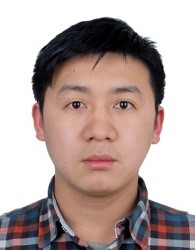
\includegraphics[width=0.4\textwidth]{./images/00.jpg}}
    %\end{sloppypar}
\end{minipage} & \begin{minipage}{0.56\textwidth}
  \raggedright
  \pinfo{尚祚彦 | Roy(Zuoyan)Shang}{1981/01/26,Nanjing}\leavevmode\\
  \wwwinfo{(+86) 13913834668}{shangzuoyan@hotmail.com}{https://shangzuoyan.github.io}
  \end{minipage}
\end{tabular}
\end{table}

 
\section{Self-assessment}
\begin{itemize}
  \setlength\itemsep{0.2ex}
  \item Proficient in \textsc{C}, \textsc{C++}, \textsc{C\#}, \textsc{Java}, \textsc{Python} and {\LaTeX} programming languages.
  \item Familiar with \textsc{TCP/IP} protocols, network programming, and proficient in design patterns.
  \item Familiar with \textsc{Qualcomm}/ \textsc{Mediatek}/ \textsc{NXP}/ \textsc{HiSilicon}/ \textsc{UniSoC}/ \\
  \hspace*{5.4em} \textsc{Rockchip}/ \textsc{Horizon}/ \textsc{BlackSesame}, \textsc{Xilinx} and \textsc{Renesas} platforms.
  \item Familiar with \textsc{Linux}/ \textsc{Android}/ \textsc{Redhat}/ \textsc{Tizen}/ \textsc{FFOS} systems.
  \item Familiar with prevailing \textsc{RTOS}(\textsc{FreeRTOS}/ \textsc{RT-Thread}/ \textsc{Nucleus}) and \textsc{microkernel}(\textsc{SeL4}/ \textsc{L4Re}/ \textsc{HelenOS}).
  \item Good system architecture design ability and embedded system programming development experience.
  \item Proficent English level, strong communication skills, and overseas work experience.
  \item Sincere, practical, hardworking, strong learning ability, and teamwork spirit.
  \item Healthy, cheerful, and responsible.
\end{itemize}
\hspace*{1.4em} \textbf{Currently working for CAIC.}
\spaceline{}

\section{Education}
\edublock{2006.09-2009.06}{Cartography and Geographic Information Systems (Master of Science)}{School of Geographical Sciences,}{Nanjing Normal University}

\edublock{1999.09-2003.07}{Industrial Design Engineering (Bachelor of Engineering)}{School of Mechanical Engineering,}{Jiangsu University}

\spaceline{}

% Comment Skills section
% \section{Skills}
% \begin{itemize}[parsep=0.2ex]
%   \item \textbf{Programing Language}: C, C++, C\#, Java, Python, Shell
%   \item \textbf{Operating System}: \textsc{Linux/ Redhat, SeL4/ L4Re/ HelenOS, FreeRTOS/ RT-Thread/ Nucleus/ QNX}
%   \item \textbf{Key words}: \textsc{GDB(Gef)}, \textsc{OllyDbg}, \textsc{Lauterbach Trace32}, \textsc{ARM}, \textsc{RSIC-V}, \textsc{QEMU}, \textsc{Gem5}
% \end{itemize}
% \spaceline{}

\section{Work Experience}
% E:1============================================================
\expblockex{2021.06-present}{Manager of Basic S/W Dept. / Operating System Specialist}{China Automotive Innovation Corperation,.Ltd[CAIC]}{Basic Software Dept., Intelligent Connected Business Unit}
\explistitemx{
  \begin{itemize}
    \item \textbf{Responsible for the design and development work of the operating system, including:}\\
  \textsc{CAIC OS}, \textsc{CAIC Hybrid OS}, \textsc{CAIC Hypervisor}, \textsc{CAIC Hypervisor Light}, and etc.\\
  The system porting works for the \textsc{NXP} i.MX8QM/ \textsc{TI} TDA4/ \textsc{MTK8675} platforms.\\
  Accomplish the functional safety \textsc{ISO 26262} certification for the \textsc{CAIC OS} and \textsc{Hypervisor}.
  \item \textbf{Some joint research and development projects:}\\
  Responsible for the \textsc{Siemens}/ \textsc{Mentor Graphics} \textsc{Nucleus} operating system cooperative project;\\
  Responsible for the \textsc{Zlingsmart} \textsc{Raite Hypervisor} cooperative project;\\
  Responsible for the lightweight virtualization system project for \textsc{Renesas} RH850/ U2A/ U2B;\\
  Responsible for the Zonal architecture \textsc{AUTOSAR} CP system on the lightweight virtualization solution;\\
  Responsible for the \textsc{Horizon Robot} J3/J5 assisted automatic driving operating system cooperative project.
  \end{itemize}
}
\spaceline{}

% E:2============================================================
\expblockex{2017.10-2021.01}{Specialized Manager of Wireless and Protocol Dept.}{FIH Communications(Nanjing) Co., Ltd}{Nanjing R\&D Center, IDM Business Unit}
\explistitemx{
  \begin{itemize}
    \item \textbf{Internal projects:}\\
  Responsible for the system porting, development, and certification works of \textsc{Sharp}(SG1/HD1/VGO/VG2) and \textsc{Nokia}(ROO/TAS) projects.\\
  Proficient in subsystems and modules such as \textsc{WLAN}/ \textsc{Bluetooth}/ \textsc{FM}/ \textsc{GNSS}, \textsc{NFC}/ \textsc{Felica}, \textsc{IR}, etc.\\
  Participated in the \textsc{Apple} ICAR Connectivity interactive scenarios project.\\
  Participated in the joint research and development works of \textsc{Byton} smart cockpit.
    \item \textbf{Outsourcing projects:}\\
  Responsible for the system porting, development, and certification works of the \textsc{Vivo} Khronos, \textsc{Xiaomi} D1S OTA/ J15s and \textsc{LG} DH0 projects.
  \end{itemize}
}
\spaceline{}

% E:3============================================================
\expblockex{2016.01-2017.10}{S/W Specialist->Director of Terminal OS Dept.}{Jiangsu HopeRun Software Co., Ltd}{Terminal OS Dept., Intelligent Terminal Business Unit}
\explistitemx{
  \begin{itemize}
    \item \textbf{Take over the AtelierOS project of Euler Laboratory in Huawei Central Software Institute:}\\
    \textsc{AtelierOS} is a virtual container based on the L4 microkernel, on which multiple operating systems can be deployed and up and running with seamless switching.\\
  Responsible for the overall system architecture design and implementation, and porting to the \textsc{Huawei Mate} series smartphones.
    \item \textbf{Take over the Texas AT\&T project of Huawei Terminal Company:}\\
  Based on the \textsc{Qualcomm} MSM8939 platform, as the project technical leader, responsible for system bringup, certification, and problem tracking.
    \item \textbf{Take over the VR project of Huawei Terminal Company:}\\
  Responsible for the system architecture and design of the project.\\
  Responsible for the development and coding works of key subsystems.\\
  Based on the restructured \textsc{gSOAP OnVIF} services, the inter-process communication service based on \textsc{LibEvent}, and the DAL encapsulation based on \textsc{SQLite}.
    \item \textbf{Take over the Smart Watch Turnkey project of ClouderSemi Company:}\\
  Responsible for the system architecture and design of the project.\\
  Responsible for the development and coding works of the system framework based on \textsc{Bluetooth}.\\
  Based on the private protocols of signaling interaction of \textsc{Bluetooth LE}, the transmission services based on \textsc{Bluetooth RF-COMM}, and the audio services of \textsc{Bluetooth HFP}/\textsc{A2DP}.
  \end{itemize}
}
\spaceline{}

% E:4============================================================
\expblockex{2013.05-2016.01}{Principal S/W Engineer->Manager of Wireless Dept.}{Yulong Computer Telecommunication Scientific(Shenzhen) Co., Ltd}{The 52rd Dept., Nanjing R\&D Center}
\explistitemx{
  \begin{itemize}
    \item \textbf{Coolpad overseas market products}\\
  Fully responsible for the connectivity related modules:\\
  \parbox[t]{3em}{\textbf{WCN:}} \parbox[t]{\textwidth-5em}{
    Bringup the integrated \textsc{WLAN}/\textsc{Bluetooth}/\textsc{FM} combo chips(WCN36\underline{X}\{1/2/6\}0).\\
    Bugshoot the issues of the certification tests, such as \textsc{WFA}/\textsc{BQB}, \textsc{BT-IOT}, and etc.\\
    Discuss the requirements with overseas operators, and analyze the field testing problems rapidly.
  }\\
  \vspace*{1.5ex}
  \parbox[t]{3em}{\textbf{GNSS:}} \parbox[t]{\textwidth-5em}{
    Configuration of WTR1605L/ WTR4905 Transceiver, SKY65611-11 PA/ eLNA chips.\\
    Solving problems in AGPS testing and SUPL1.1/ 2.0 certification testing.
  }\\
  \vspace*{1.5ex}
  \parbox[t]{3em}{\textbf{NFC:}} \parbox[t]{\textwidth-5em}{
    Bringup the \textsc{NXP} PN544/PN547 chips, driver debugging, NFC protocol stack upgrade, SmartCard solution integration, 
    \textsc{EMVCo2.3.3} certification, and support for \textsc{VISA}/ \textsc{MASTERCARD}/ \textsc{AMEX} payment.
  }\\
  \vspace*{1.5ex}
  \parbox[t]{3em}{\textbf{IR:}} \parbox[t]{\textwidth-5em}{
    Bringup the \textsc{ABOV} MC96FR116CU chips, and driver debugging.\\
    Finish the development works of new requirements of \textsc{TMO} operators, including DeviceReporting, HW Encyption, Anti-theft Feature, and etc. 
  }
    \item \textbf{Related platforms involved are as follows:}\\
  \hspace*{3em} MSM8926 (\textsc{Vodafone Smart 4 Max})\\
  \hspace*{3em} MSM8916 (\textsc{Panasonic ELUGA L 4G})\\ 
  \hspace*{3em} MSM8909 (\textsc{China Mobile Y75})\\
  \hspace*{3em} MSM8939 (\textsc{Qikoo}), etc.
  \end{itemize}
}
\spaceline{}

% E:5============================================================
\expblock{2009.10-2013.05}{Sr. S/W Engineer->Manager of S/W Dept.}{TeleEpoch Co., Ltd}{Software Dept., Nanjing R\&D Center}
\explistitemx{
  \begin{itemize}
    \item \textbf{Qualcomm AMSS8960/AMSS8625 projects:}\\
  Responsible for the modem side software, 
  and undertake the implementation of the telephony-related code in the Android Framework/RIL and QCRIL layers.
    \item \textbf{Qualcomm AMSS7627 F3610/F3611 projects:}\\
  Responsible for the modem side software, 
  Responsible for the related code implementation in the Android Framework/RIL and QCRIL layers, and responsible for the IOT Level2 test (Fort Worth, Texas, Motorola network laboratory).
    \item \textbf{Qualcomm QSC6085 CDMA 1x EVDO M600 project:}\\
  Responsible for the MMS, WAP browser, and WWW (Full HTML) browser modules, 
  and was responsible for the MMS/WAP IOT test (Fort Worth, Texas, Motorola network laboratory), and discussed functional requirements and technical support matters with PCD, UMX, and US Cellular.
    \item \textbf{Qualcomm QSC6055 CDMA 1x WMDP project:}\\
  Responsible for the application modules of automatic speech recognition [ASR] (\textsc{iFlyTek}/ \textsc{VoiceSignal Tech}), 
  and gravity sensor [G-Sensor]. Exhibited at CES2010 and the Asia Telecom Exhibition.
    \item \textbf{Qualcomm QSC6270 GSM/WCDMA(DSDS) projects:}\\
  Undertake the low-level driver works, including: \\
  \hspace*{3em} \ding{172} \textsc{FLASH} driver (\textsc{Micron}/ \textsc{Hynix}).\\
  \hspace*{3em} \ding{173} \textsc{LCD}/ \textsc{MDP} driver (\textsc{Sunrise}/ \textsc{Truly}, IC: TM2.0/3.55 ILI9341/9225/9225G HX8340B/8347D).\\
  \hspace*{3em} \ding{174} \textsc{T9}/ \textsc{QWERTY} keyboard driver. \\
  \hspace*{3em} \ding{175} \textsc{HALL} device flip device driver.\\
  Undertake the underlying implementation works of \textsc{GSDI} dual-card support.\\ 
  Undertake the works of the \textsc{OEM} interface layer and the application layer.\\ 
  Responsible for the modules such as: \textsc{SMS} (\textsc{GSM 03.38}/ \textsc{03.40}/ \textsc{07.05}), \textsc{MMS} (\textsc{TS23.140}/ \textsc{OMA}), 
  \textsc{STK} (\textsc{GSM 11.14}), \textsc{SIM} card (\textsc{TS 31.102}), \textsc{Bluetooth}, \textsc{Brew JavaVM}, \textsc{WWW} (Full \textsc{HTML}) browser, \textsc{Multimedia}, and \textsc{Input Method Engine}.
    \item \textbf{Qualcomm MDM6085 CDMA 1x EVDO D2/D3/D5 data card projects:}\\
  Responsible for the development and debugging tasks of the lower computer AT commands and the upper computer synchronization and dialing software.
  \end{itemize}
}
\spaceline{}

% E:6============================================================
\expblockex{2006.07-2009.05}{Graduated Student}{National Key Laboratory of Virtual Geographic Environment[VGEKL]}{Ministry of Education + Nanjing Normal University (NJNU)}
\explistitemx{
  \begin{itemize}
    \item \textbf{Research on the key technologies of 3D GIS for space entities based on the non-manifold theory}\\
Project Number: \textsc{2007AA12Z236} [National 863 Project][2007.11-2009.05]\\
Engaged in the researchs of:\\
\hspace*{3em} \ding{172}3D GIS framework based on \textsc{OSGi RCP}.\\
\hspace*{3em} \ding{173}Spatial data indexing: the general search tree \textsc{GiST}, Space Index Library, and hybrid index \textsc{OR-tree}.\\
\hspace*{3em} \ding{174}Data visualization: \textsc{Open Inventor}, \textsc{IRRLicht}, \textsc{OSG}, \textsc{Coin3D}.\\
Responsible for the development tasks of the prototype system.
    \item \textbf{Research on the key technologies for the copyright protection of GIS vector data products}\\ 
Project Number: \textsc{2006AA12Z222} [National 863 Project][2006.10-2007.03]\\
Engaged in the researchs of:\\
\hspace*{3em} \ding{172}\textsc{pseudo-random sequences}: \textsc{M-sequence}, \textsc{golden sequence}, and \textsc{chaotic sequence}.\\
\hspace*{3em} \ding{173}\textsc{watermark} embedding and extraction.\\
\hspace*{3em} \ding{174}\textsc{wavelet} decomposition and reconstruction.\\
Engaged in the algorithm implementation of watermark embedding in and extraction from high-dimensional space data, and participated in the development tasks of the prototype system.
  \end{itemize}
}
\spaceline{}

% E:7============================================================
\expblock{2003.10-2006.08}{S/W Engineer}{AMOI Electronics Co., Ltd}{Communication Dept., Nanjing Research Institute}
\explistitemx{
  \begin{itemize}
    \item \textbf{Related platforms and operating systems:}\\
    \textsc{Spreadtrum} platform, \textsc{X-Thread} RTOS.\\
    \textsc{Qualcomm} platform, \textsc{Rex} OS/ \textsc{Brew}/ \textsc{BrewMP} systems.\\
    \textsc{Toshiba} platform, \textsc{iTRON} system.
    \item \textbf{Responsibilities in the project:}\\
  Mainly responsible for the software development tasks of the \textsc{PHS} and \textsc{Smartphone}.\\
  \textsc{MMI} driver, \textsc{LCD} driver, functional business modules(\textsc{PIM}/\textsc{PIN}, \textsc{Phonebook}, and \textsc{Schedule}), and application programs.\\
  Accumulated rich project development experience, became familiar with the protocols and file structure of \textsc{PIM}, and had an in-depth understanding of the \textsc{iTRON} system. \\
  And served as the software group leader in the \textsc{PHS S368} project. 
  \end{itemize}
  % Responsible for the overall planning of the software development tasks of the entire project and software version control.\\
}
\spaceline{}

%\hspace*{4em}\parbox[c]{\textwidth-4em}{ }


% ============================================================
\section{Publications and Commitments}
% increase linespacing [parsep=0.5ex]

\textbf{Co-author of 3 publications}

[1] Xu H, Lu G, Sheng Y, Guo F, \textbf{Shang Z}.3D GIS spatial operation based on extended Euler operators[J].\newline
  Proceedings of SPIE - The International Society for Optical Engineering, 2008, 7143:71433D-71433D-10.\newline
  DOI:10.1117/12.812655.\newline
[2]\textbf{尚祚彦}.3D GIS混合空间索引技术研究[D].南京师范大学,2009.DOI:10.7666/d.d183065.\newline
[3]张璐,柴燕妮,王丹,\textbf{尚祚彦}.基于地理国情的县域生态环境质量评价研究[J].地理空间信息, 2022, 20(10):79-81.

\textbf{Co-inventor of 5 patents}
\vspace{0.6ex}{}

\setlength{\extrarowheight}{0.8ex}

\begin{tabularx}{\textwidth}{m{7.2em}|X|m{6.6em}}
\hline
\makecell[lt]{Patent Number} & \makecell[lt]{Patent Description} & \makecell[lt]{Publication Date}\\
\hline
[CN115480934A] & 专利一种分布式数据处理的方法、装置、设备及储存介质 & 2022/12/16\\
\hline
[CN114153560A] & 专利一种虚拟中断处理方法、装置、设备及介质 & 2022/03/08\\
\hline
[CN114579556A] & 专利一种数据处理方法、装置、设备及存储介质 & 2022/06/03\\
\hline
[CN114579556B] & 专利一种数据处理方法、装置、设备及存储介质 & 2022/08/02\\
\hline
[CN114298990A] & 专利一种车载摄像装置的检测方法、装置、存储介质及车辆 & 2022/04/08\\
\hline
[CN114500408A] & 专利一种以太网络交换装置、数据处理装置和车辆 & 2022/05/13\\
\hline
\end{tabularx}




  
  


%% Reference
%\newpage
%\bibliographystyle{IEEETran}
%\bibliography{mycite}
\end{document}
